% ==============================================================================
% POSTER STYLE DON'T MODIFY
\documentclass[final]{beamer}
\setbeamertemplate{caption}[numbered]
\beamertemplatenavigationsymbolsempty

\usepackage[orientation=portrait,size=a0,scale=1.25]{beamerposter}
\usepackage[utf8]{inputenc}
\usepackage[T1]{fontenc}
\usepackage{tikz}
\usepackage{lmodern}
\usepackage{amsmath,amsthm, amssymb, latexsym}
\usepackage{url}
\usepackage{ragged2e}
\usepackage{parskip}

\usepackage{algpseudocode}
\usepackage{algorithm}
\MakeRobust{\Call}

\usepackage{multicol}
\setlength{\columnsep}{80pt}

\usepackage{graphicx}
\usepackage{listings}

% used for drawing section lines etc...
\usepackage{tikz}
\tikzset{every mark/.append style={scale=3.5}}
\usepackage{pgfplots}
\usepackage{pgfplotstable}
\pgfplotsset{	
	compat=newest,
	width=7.5in,
	max space between ticks=100pt,
	every axis plot post/.append style={ultra thick},
	/pgfplots/ylabel absolute/.style={%
		/pgfplots/every axis y label/.style={at={(0,0.5)},xshift=4em,rotate=90},
		%/pgfplots/every y tick scale label/.style={
		%at={(0,1)},above right,inner sep=0pt,yshift=0.3em
		%},
	},
}

\linespread{1.05}
\geometry{hmargin=2.5cm}

% define basic colors
\definecolor{black}  {RGB}{0,0,0} 		%%% text color
\definecolor{blue}  {RGB}{20,66,129} 		%%% title and subsection color
\definecolor{lightblue}  {RGB}{28,130,185} 	%%% section color
\definecolor{lightgrey}  {RGB}{255,253,250} 	%%% background color

\setbeamercolor{structure}{fg=blue}
\setbeamercolor{colorbar}{fg=black,bg=blue}
\setbeamercolor{normal text}{fg=black}
\beamertemplatesolidbackgroundcolor{lightgrey}

%set bibliography style
\setbeamertemplate{bibliography item}[text]
\setbeamercolor{bibliography item}{fg=black,bg=lightgrey}
\setbeamercolor{bibliography entry author}{fg=black,bg=lightgrey}
\setbeamerfont{bibliography item}{size=\small}
\setbeamerfont{bibliography entry author}{size=\small}

% poster title
\setbeamertemplate{headline}{
  \leavevmode
  \vskip 2cm
  \begin{columns}
    \begin{column}{0.15\linewidth}
      \begin{center}
        %\includegraphics[width=0.55\linewidth]{logo}
      \end{center}
    \end{column}
    
    \begin{column}{.7\linewidth}
      \centering{
        {\color{lightblue}
        \setlength\lineskip{20pt}
        \textbf{\huge{\inserttitle}}\\[1ex]}
      	\vskip 1cm
        {\color{fg} \Large{\insertauthor}\\[1ex]}
        {\color{fg} \large{\insertinstitute}\\[1ex]}
      }
      \vskip 1cm
    \end{column}
    
    \begin{column}{.15\linewidth}
      \begin{center}
        %\includegraphics[width=\linewidth]{eda-logo}
      \end{center}
    \end{column}

    %%%\vspace{5cm}
  \end{columns}
}

% poster foot
\setbeamertemplate{footline}{
  \leavevmode
  %\vskip 1cm
  
  % horizontal line
  \begin{flushleft}
    \begin{tikzpicture}[remember picture,overlay]
      \shade [inner color=lightblue,outer color=lightgrey] (0,0) rectangle (\textwidth,0.3cm);
    \end{tikzpicture}
  \end{flushleft}
        
  \vskip 1cm
        
  \begin{center}
    \begin{columns}[c]
	  \begin{column}{0.1\linewidth}
	    \begin{center}
	      %\includegraphics[width=6cm]{rma_1600.png}
	    \end{center}
	  \end{column}
	    
	  \begin{column}{.4\linewidth}
	    \begin{center}
	      %\includegraphics[width=6cm]{EURECOM_logo_quadri.pdf}
          \color{lightblue}
          \setlength\lineskip{20pt}
          \textbf{\Large{Cyber Defence Lab\\}}
          \large{Royal Military Academy\\
          \url{www.cylab.be}}
	    \end{center}
	  \end{column}
	    
	  \begin{column}{.1\linewidth}
	    \begin{center}
           %\includegraphics[width=6cm]{symantec-logo-300dpi.png}
	    \end{center}
      \end{column}
    \end{columns}
  \end{center}
  
  \vskip 1cm
}

% Section
\renewcommand{\section}[1]{
    % horizontal line
    %\par\vskip\medskipamount%
    %\begin{flushleft}
    \begin{tikzpicture}[remember picture,overlay]
      \shade [inner color=lightblue,outer color=lightgrey] (0,0) rectangle (\columnwidth,0.3cm);
    \end{tikzpicture}
    %\end{flushleft}
    
    \vskip 1.25cm

    \begin{center}
      %\vskip1cm
      \textcolor{lightblue}{\textbf{\Large #1}}
      %\parskip0pt\par
    \end{center}

    %\begin{flushleft}
    \vskip 0.25cm
    
    % horizontal line
    \begin{tikzpicture}[remember picture,overlay]
      \shade [inner color=lightblue,outer color=lightgrey] (0,0) rectangle (\columnwidth,0.3cm);
    \end{tikzpicture}
    %\end{flushleft}
    
    \parskip 10pt \par
    \justifying
}

%%% Sub-section
\renewcommand{\subsection}[1]{
  %\par\vskip\medskipamount%
  %\begin{center}
  \vskip 1.2cm
  \textcolor{lightblue}{\textbf{\textsl{\large #1}}}
  %{\parskip0pt\par}
  %\end{center}
  \justifying
}

% ==============================================================================
% Title, date and authors of the poster
\title{Smart Router}

\author[shortname]{
	Thibault Debatty \inst{1} \and
	Pietro Michiardi \inst{2} \and
	Olivier Thonnard \inst{3} \and
	Wim Mees \inst{1}
}
\institute[shortinst]{
	\inst{1} Royal Military Academy, Brussels, Belgium \and
  \inst{2} EURECOM, Campus SophiaTech, France \and
  \inst{3} Symantec Research Labs, Sophia Antipolis, France
}



% ==============================================================================
% Content of the poster

\usebackgroundtemplate{%
\tikz\node[opacity=0.1] {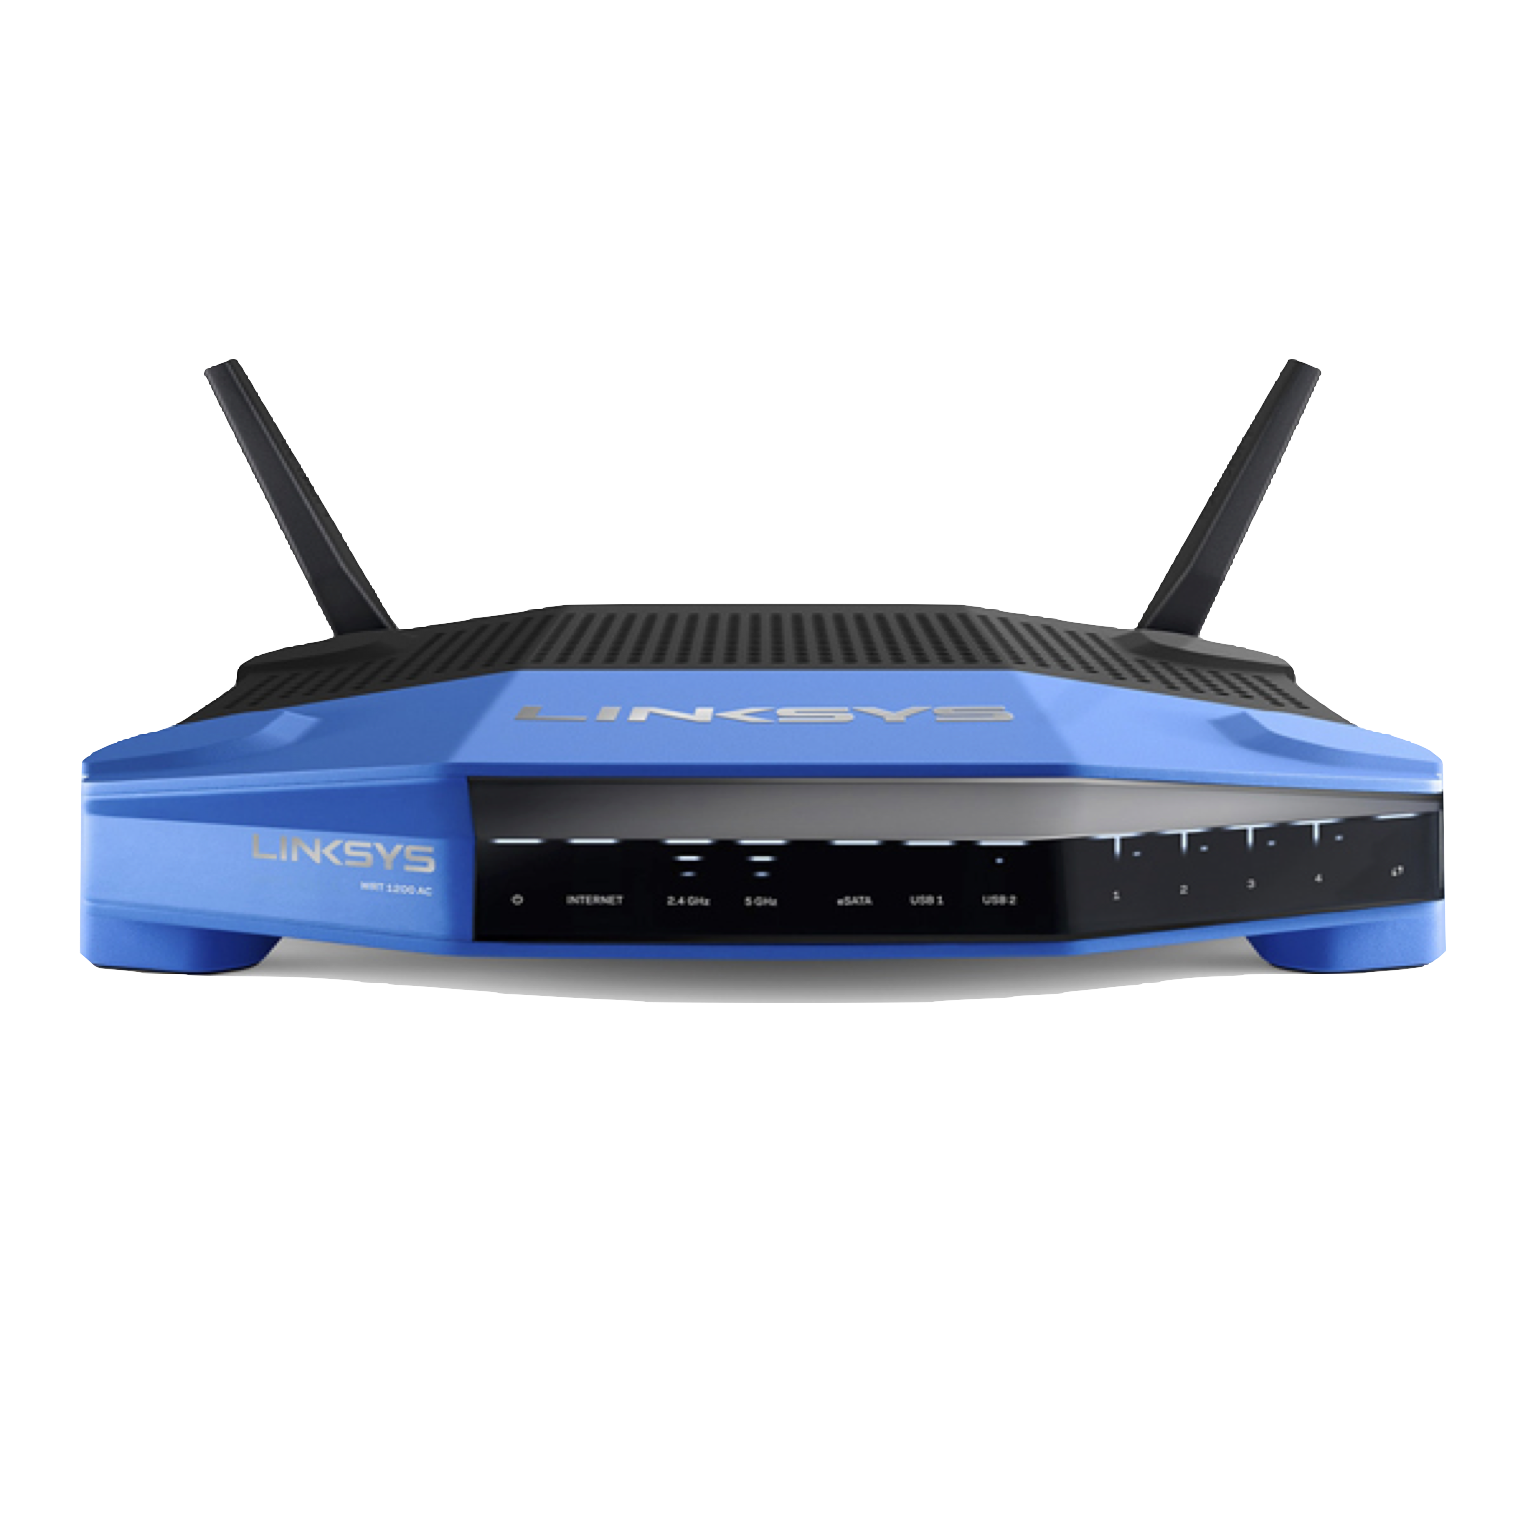
\includegraphics[height=\paperheight,width=\paperwidth]{Pictures/wrt1200ac.png}};}




\begin{document}
\begin{frame}{}
\begin{multicols}{3}



\section{Introduction}
The number of IoTs devices present in our houses is constantly growing up. Smart-TVs, smart-lights,IP-cameras and number others are all connected to the Internet to be managed from outside our homes. But how can we, in as SOHO context, monitor these devices to be sure they only do the work they should. So how to be sure they are not botnets ? 

\subsection{Goal}\\
The goal of this project is to monitor IoT traffic of a SOHO (Small Office, Home Office) network. By monitoring it, this project can send alerts when an IoT has an unusual network traffic. For example, if it suddenly begin to send random request to random IP addresses around the world.


\section{Structure}
This project was initially designed from Ubuntu machine but was then adapted to work on an OpenWRT distribution which is more adapted from network embedded devices. This project was developed in Python3.

\subsection{Design}\\ 
The design of the router is the next one : 
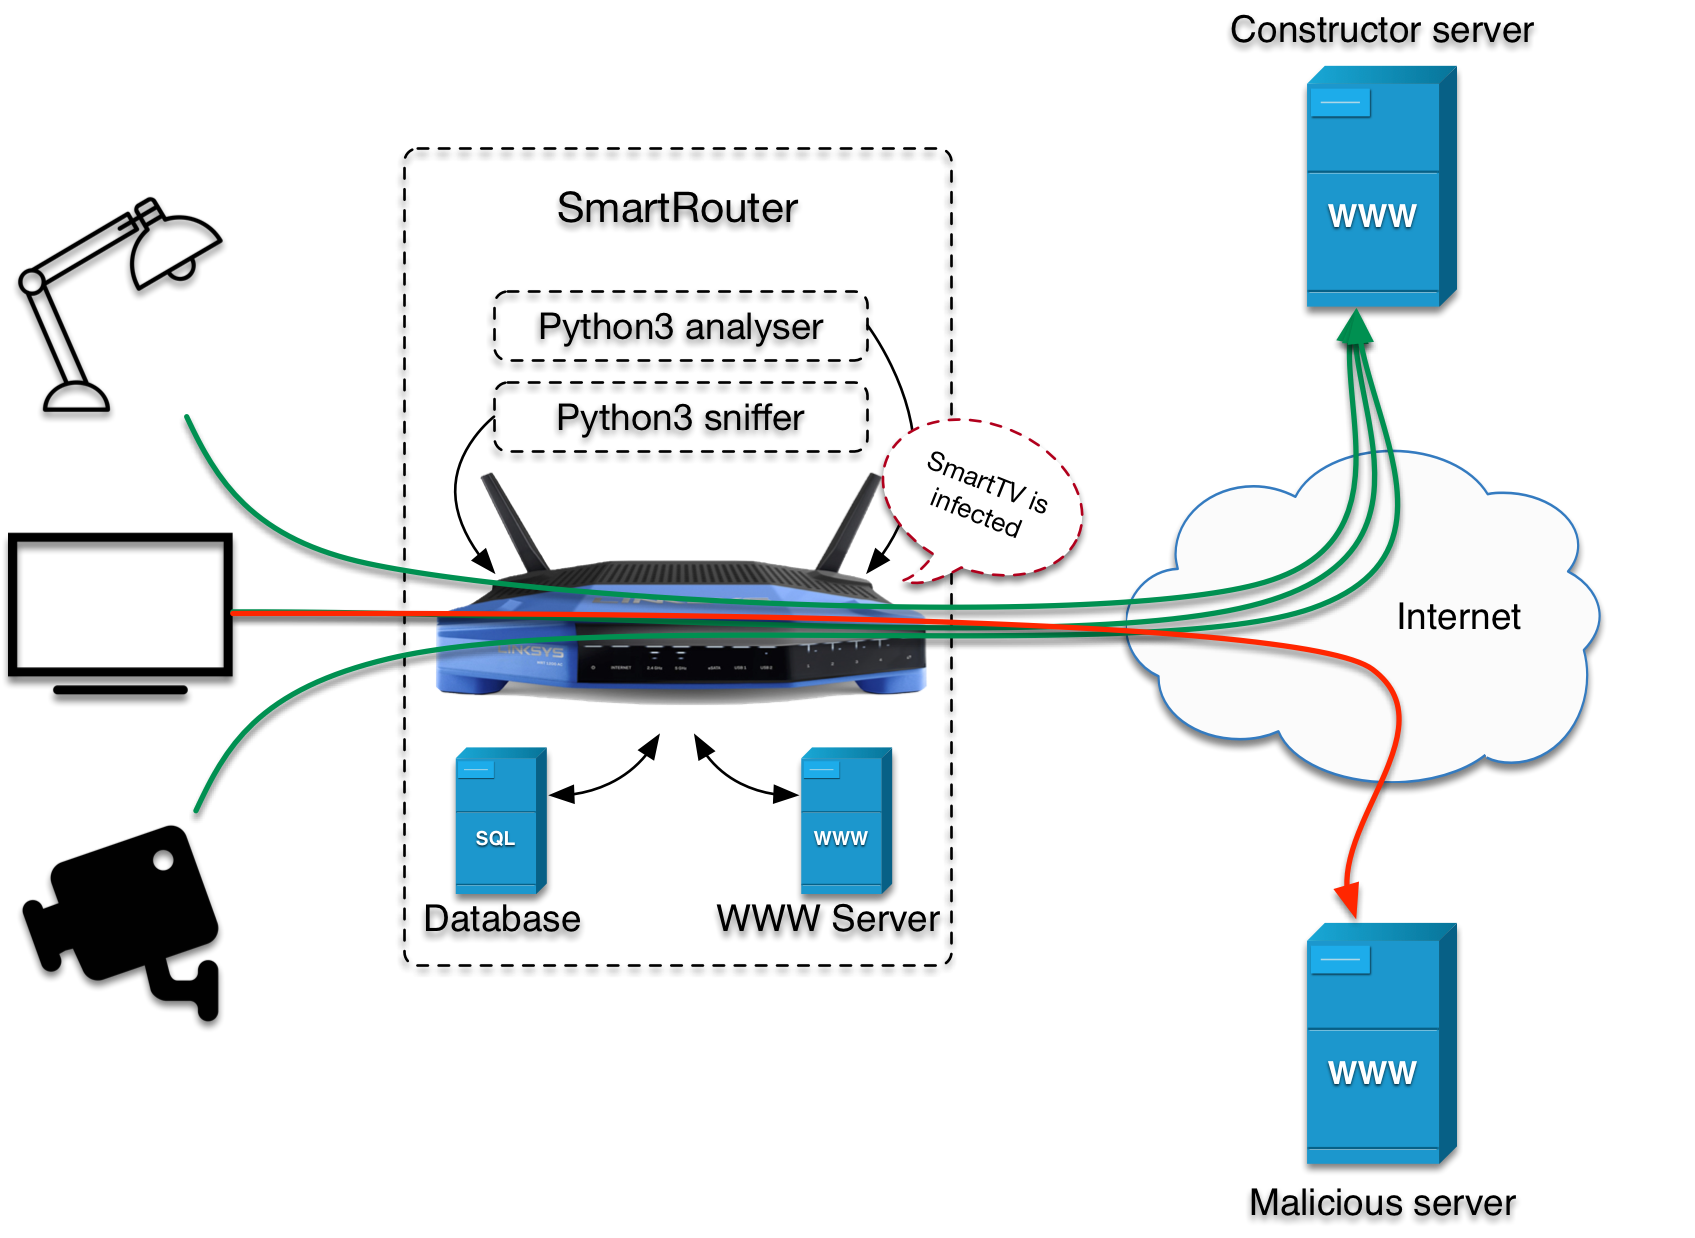
\includegraphics[width=0.35\textwidth]{Pictures/design.png}


\subsection{OpenWRT $^{(\text{\url{https://openwrt.org}})}$}\\
The OpenWrt Project is a Linux operating system targeting embedded devices. So it was one of the possible choices for the Linux distribution. More specifically, OpenWRT was a compatible distribution for the router used for this project. The routers used are Linksys WRT1200ac.

\subsection{Scapy}\\
The main goal of the project is to have a router which executes 2 main tasks :
\begin{itemize}
  \item Sniff : all SYN packets of TCP/80 \&\& TCP/443 are sniffed and stored in an SQLite3 database. To be able to know which IP corresponds to which domain, DNS packets are also sniffed and then data are correlated to make IP correspond to a domain. If no domain corresponds to an IP, IPs are DNSreversed to try to have a domain. 
  \item Analyze : after having sniffed packet, a process must be launched to analyze all traffic and determine if the traffic is legit or malicious.
\end{itemize}




\section{Installation}
The installation is very simple thanks to auto-deploy scripts. A Readme is present to the Github the guide the installation. 

Like routers used for this project do not have a lot of storage, a USB stick is needed to expand data storage. All this procedure is also explained in the Github(\url{https://github.com/RUCD/smart-router}).


One of the auto-deploy script is the following :

sh -c "\$(curl -fsSL https://raw.githubusercontent.com/\\
RUCD/smart-router/master/docs/setupScripts/setupSR.sh)"


\section{Alerting}
Initially, two different types of alerting had been designed. On via a web browser, and another one, optional, like an application or something like that. 

\subsection{Slack alerts}\\
Slack alert have the role of the initial application alert. A slack application has been integrated in a workspace. So with it, the Smart Router send alert to a specific channel, thanks to slack tokens. 

This slack integration allow the receive notification like initially wanted, but without having to develop a specific application for it.

\subsection{Web server}
A web server using Laravel framework was initially designed to assure the web server role. But due to portability issues and high resource consumption, alert are simply read on a text file and displayed vie a simple web server.

\section{Future Work}
Lots of modules can be developed in future work, for example we can imagine : 
\begin{itemize}
	\item More protocol sniffed : for now, only web and DNS traffic is sniffed, but it could be interesting to have a generic sniffer which allowed to sniff everything traffic,
	
	\item Web configurations : all configuration is done in command line, so a more user-friendly web interface configuration page could be a great idea,
	
	\item Target sniffing : a good idea will be to be able to detect IoTs and filter only this traffic. Actually, all traffic is sniffed, but some can be blacklisted not to be sniffed,

	\item Target analysis : actually, all traffic is reanalyzed every time an analysis is run. A better analysis will be to analyze only new traffic since the last analysis,

	\item Lots of other integration are possible to have better interfaces and configuration modules.
\end{itemize}
% more protocols sniffed
% web server 


\section{Conclusion}
This project has a lot of other possibilities then experimented here. It also has a lot of optimization and machine learning possible. 

\end{multicols}
\end{frame}
\end{document}










